En el Capítulo \ref{chapter_fenomeno} revisamos cómo un pulso de 
radiofrecuencia (RF), sintonizado a la frecuencia de Larmour $\omega_0$ es 
capaz de perturbar el momento magnético del sistema de spins (\M). Si la 
radiofrecuencia se aplica durante un tiempo determinado, podemos desviar a \M
a nuestro gusto. A esto le llamamos 
\textit{excitación}. Si provocamos una desviación de 90\degrees, \M
pasará de estar totalmente en el eje $z$ (\Mz=\M) al plano $x,y$, mientras que una  desviación de menos de 90\degrees ($\alpha$\degrees) colocará una fracción de \M en el plano $x,y$ (específicamente, $\sen(\alpha)$).

Una vez que el pulso de RF se apaga, el sistema de spins tenderá a regresar a 
su estado de reposo, es decir, sobre el eje $z$ (alineado con \Bzero). Este 
regreso al estado de reposo se conoce como \textit{relajación} y es la causa principal por la que nuestra señal es abundante al principio y progresivamente desaparece en un decaimiento libre (\textit{free-indiction decay}, FID)\index{FID}. Mientras  \M tenga una proyección sobre el eje $x,y$, estaremos recibiendo señal de resonancia, y ésta última irá decayendo poco a poco, porque \M estará regresando a apuntar al eje $z$, disminuyendo progresivamente su proyección en el eje $x,y$. Si tuviéramos una muestra exclusivamente de 
Hidrógeno (sin impurezas), en un campo magnético perfectamente homogéneo, todos 
los átomos de H se relajarían al mismo ritmo, emitiendo señal perfectamente 
sintonizada a $\omega_0$. Esto sería un experimento aburrido, pues la RF que 
inyectamos, sintonizada a $\omega_0$ sería exactamente la misma que 
recibiríamos. Afortunadamente, en el mundo real no sucede así, y la relajación 
de diferentes tejidos sucede a diferentes velocidades. Al realizar la obtención 
de la señal, podemos permitir que pase cierto tiempo a partir de la excitación, 
con lo que permitiremos que los diferentes tejidos se relajen en distintas 
proporciones. La señal que recibiremos de cada uno de ellos será 
distinta: algunos tejidos se habrán relajado tanto que su proyección en el 
plano $x,y$ será casi nula, mientras que aquéllos que tarden mucho en relajarse 
podrán emitir mucha señal. A esta diferencia de intensidad de señales se le 
conoce como \textit{contraste}, y en términos de imagen provoca que algunos 
pixeles sean más brillantes que otros.

Existen dos fenómenos de relajación  que son independientes, pero que 
suceden simultáneamente. Esto en ocasiones provoca confusión, pero es análogo a 
lo que sucede con los fenómenos de rotación y traslación de nuestro planeta. A 
continuación describiremos los dos tipos de relajación.

\section{Relajación longitudinal: \Tone}
\index{T1|textbf}
Comencemos con una excitación con $\alpha$=90\degrees que provoca que \M se 
sitúe por completo en el plano $x,y$, precesando alrededor de \Bzero (que está 
en el eje $z$). Al apagarse el pulso de RF, \M precesa alrededor de \Bzero, y 
 progresivamente se volverá a alinear al eje $z$. En este periodo de tiempo, \M 
parecerá ``levantarse'' del plano $x,y$, mientras continúa rotando alrededor de $z$, provocando una trayectoria espiral ascendente (Figura \ref{fig:T1}) que recuerda a un helado de McDonald's. En tejido vivo, utilizando campos magnéticos de uso clínico (1 a 7 teslas), la relajación longitudinal \Tone sucede a lo largo de segundos. 


\begin{figure}[htb]
\begin{figg}
   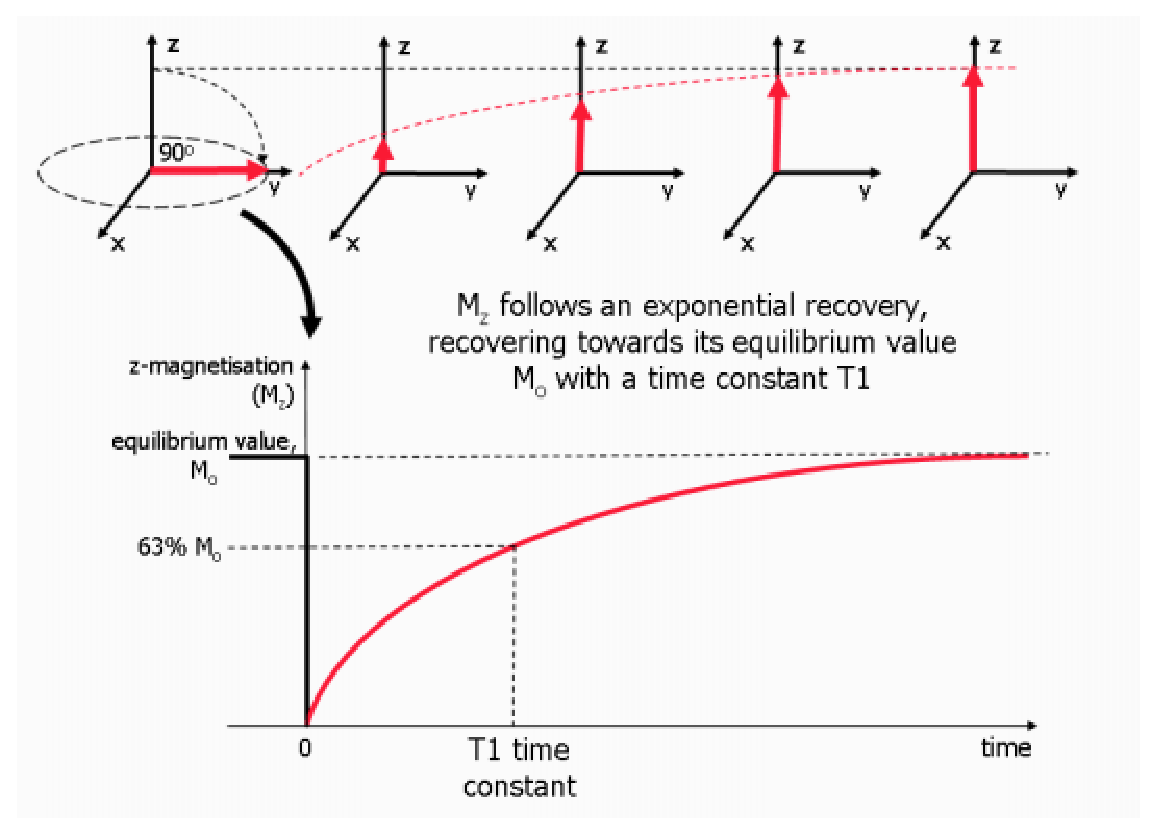
\includegraphics[width=0.7\textwidth]{contraste_T1}
   \caption{Relajación \Tone. Imagen provisional tomada de la tesis de Sasidhar Tandaki. \citep{tadanki2018}}
 \label{fig:T1}
 \end{figg}
\end{figure}



Conforme \M regresa a apuntar al eje $z$, su proyección sobre dicho eje aumenta progresivamente, y ésto es independiente de hacia qué dirección está apuntando. En otras palabras, cuando hablamos de \Tone, solo nos importa su proyección sobre $z$, que denotaremos con \Mz. Designemos a \Mzero como el la magnitud inicial de \M (antes de nuestro pulso de RF, con el sistema de spins intacto). Dada nuestra excitación con 90\degrees, entonces \Mz vale cero justo después de apagar el pulso de RF, y comienza a crecer hasta que \Mz = \Mzero. No puede crecer más que \Mzero, pues no puede haber más spins que con los que comenzamos. La manera en que \Mz crece tiene una forma peculiar: describe una curva exponencial ascendente (Figura \ref{fig:T1}) que se engloba como
\begin{equation}
\label{eq:Tone}
 M(t) = M_0(1 - e^{-\tau/T1})
\end{equation}
donde $\tau$ indica el periodo de tiempo entre pulsos de RF sucesivos. En nuestro ejemplo, solo hemos utilizado un pulso de RF, así que lo ignoraremos por ahora, pero será importante más adelante.  \Tone es el parámetro principal que le da la forma a la curva exponencial. Es el parámetro que hace que suba más rápida o lentamente, y se mide en unidades de tiempo (s). Mientras más corto es \Tone, la curva sube más rápidamente, mientras que valores largos de \Tone harán que la curva ascienda perezosamente. Revisando la Figura \ref{contraste_T1} y despejando la ecuación \ref{eq:Tone},  podemos darle una intuición sencilla a \Tone como ``el tiempo en que tarda en recuperarse el 67\% de \Mzero''. Insistimos: si \Tone es largo, \Mz tarda mucho en ``crecer'' sobre el eje $z$. 

La eficiencia con la que un tejido transfiere a su entorno el exceso de energía depositado en él mediante la RF determina su tasa de relajación longitudinal, por lo que esta relajación se conoce también como spin-matriz o \textit{spin-lattice}. La grasa y la substancia blanca (repleta de lípidos), por ejemplo, son altamente eficientes en esta transferencia de energía, mientras que el agua libre de los ventrículos cerebrales lo hace lentamente (Figura \ref{fig:contraste_T1_tejidos}).

\begin{figure}[htb]
\begin{figg}
   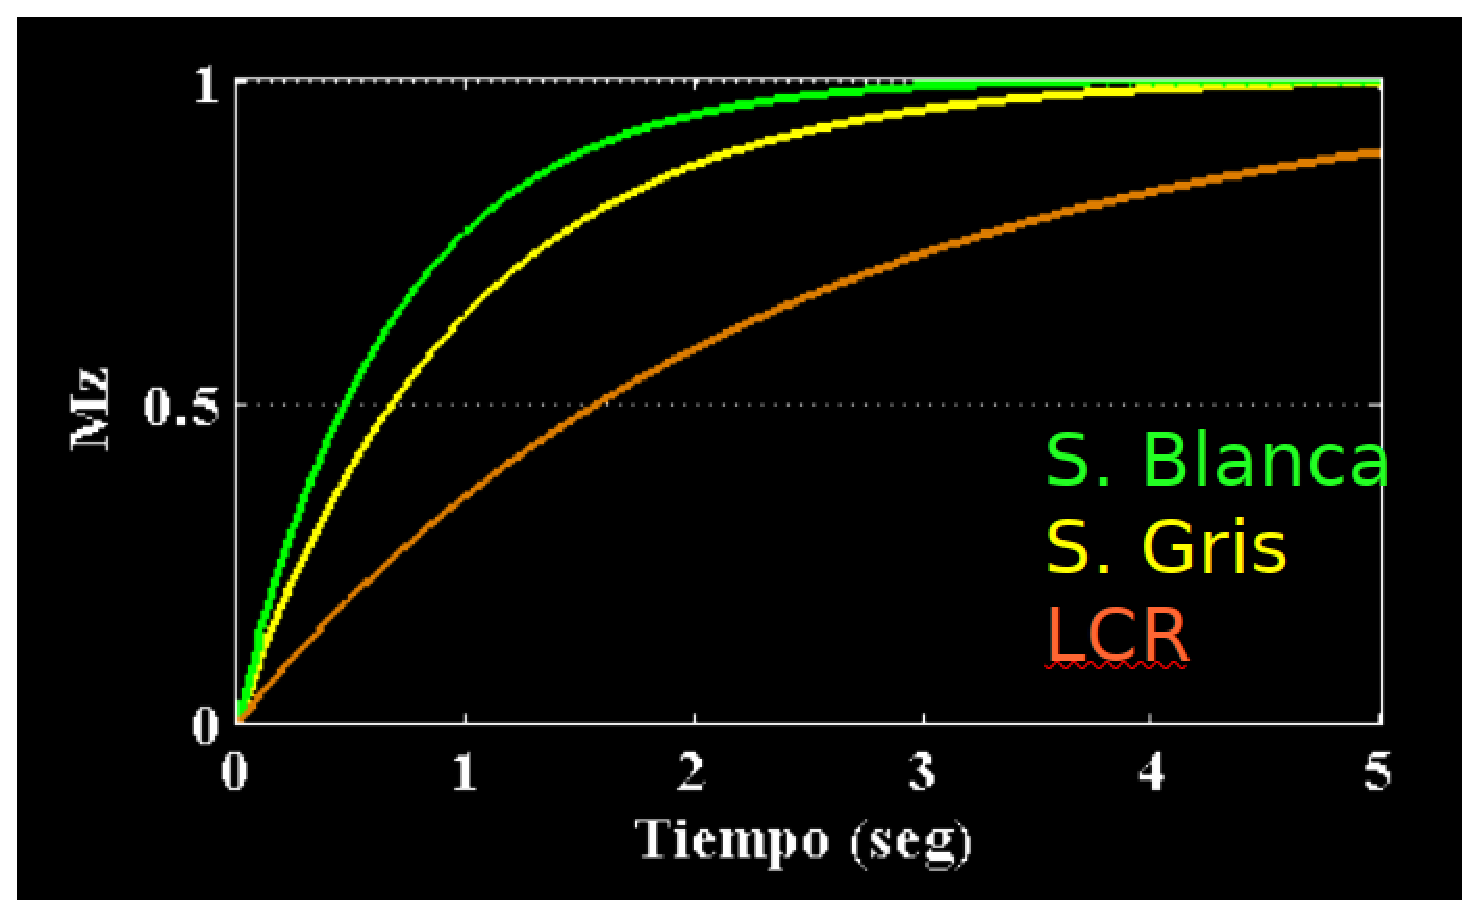
\includegraphics[width=0.7\textwidth]{contraste_T1_tejidos}
   \caption{Diferentes tejidos tienen diferentes tasas de relajación longitudinal \Tone. En el cerebro adulto, la substancia blanca presenta la relajación longitudinal más acelerada; por el contrario, el líquido cerebro-raquídeo (LCR) disipa el exceso de energía lentamente y presenta una relajación longitudinal lenta, con un \Tone largo.}
 \label{fig:contraste_T1_tejidos}
 \end{figg}
\end{figure}


\section{Relajación transversal: \Ttwo}
\index{T2|textbf}
Para poder describir este tipo de relajación, debemos recordar que \M es el vector resultante de la suma de muchas barras magnéticas ($\mu$) asociadas a cada uno de los protones de H (ver Capítulo \ref{chapter_fenomeno}). Cuando estuvo prendido el pulso RF, todos estos pequeños imanes $\mu$ se alinearon con \Bone, es decir, la radiofrecuencia. Si el pulso de RF fue de 90\degrees, todos estarán ahora alineados en algún lugar del plano $x,y$. Todos apuntan al mismo sitio, y si los vemos desde arriba (volteando a ver el plano $x,y$), estarán todos ``apilados''. La suma vectorial de muchos pequeños vectores que apuntan en la misma dirección y sentido resulta en un vector de gran magnitud, con la misma dirección y sentido. Esto es similar a cuando varios niños jalan de una cuerda: aunque cada niño tenga poca fuerza, la suma de todas sus fuerzas será tal que podrían jalar un auto. En un escenario perfecto, \M se relajaría únicamente por la influencia de \Tone, porque todos los spins precesan perfectamente a la misma frecuencia. En el mundo real, en el tejido que estamos analizando, existen pequeñas imperfecciones del campo magnético que experimentan los distintos spins. Consideremos un pixel en un sitio anatómico, por ejemplo el tálamo, en el cerebro. Un pixel tiene dimensiones de alrededor de 1 mm por lado, donde pueden caber muchísimas neuronas, células gilales, capilares sanguíneos, etc. La composición molecular y atómica de todas estas estructuras es variada, y pueden contener elementos que interaccionan con el campo magnético principal \Bzero, por ejemplo el Fe que está en la hemoglobina de la sangre, o el Cu que suele acumular el tálamo a lo largo de la edad. Si nuestro voluntario está en un resonador de 3 teslas, a nivel microscópico existirán pequeñas desviaciones de 3 teslas, haciendo que algunos spins experimenten un poco más de 3 teslas, mientras que otros (en el mismo pixel, pero unos micrómetros más alejados de los primeros) experimenten un poco menos de 3 teslas. 


Recordemos que la frecuencia de precesión \omegazero de los protones de H depende únicamente del campo magnético \Bzero que experimentan. Las variaciones intra-pixel de \Bzero son muy pequeñas (microteslas), pero provocan que cada grupo de spins precese a distintas frecuencias. Las diferencias de frecuencias entre los diferentes spins son muy sutiles, pero reales. Esto va a traducirse que, una vez que el pulso de RF se apague, los spins que precesan más rápido ``se adelanten`` a los que precesan más lento. Con el paso del tiempo, veríamos que los spins que componen a \M comienzan a \textit{desfasarse} entre ellos. Mientras más se desfasen, la suma vectorial de ellos tenderá a cero, y \M irá desapareciendo. Como se revisó en la sección \ref{section:mrsignal}, la señal que obtenemos requiere que \M esté en el plano $x,y$, y si \M va desapareciendo, nuestra señal entonces también.

La curva que describe la señal a lo largo del tiempo es exponencial, pero en este caso decreciente (Figura \ref{fig:T2}), y descrita como:

\begin{equation}
\label{eq:T2}
 M_{xy}(t) = M_{xy,max} (e^{-t/T2})
\end{equation}

donde $M_{xy,max}$ es la magnitud del componente de \M que se encuentra en el plano $x,y$ justo después de la excitación (la cantidad máxima de señal que podemos obtener tras la excitación y, en el caso de una desviación de 90\degrees, sería igual a \M). En el exponente vemos a $T_2$, que está dictando la forma de la curva exponencial, y se mide en unidades de tiempo (s). Si \Ttwo es largo, entonces la señal se pierde lentamente; si es corto, en poco tiempo habremos perdido nuestra señal. Intuitivamente, \Ttwo es el tiempo al cual solamente queda el 37\% de la señal \Mxy original. Finalmente, $t$ indica en qué momento estamos valorando cuánta señal hay, y será un parámetro que podremos explotar más adelante para extraer más o menos contraste tipo \Ttwo. 

\begin{figure}[htb]
\begin{figg}
   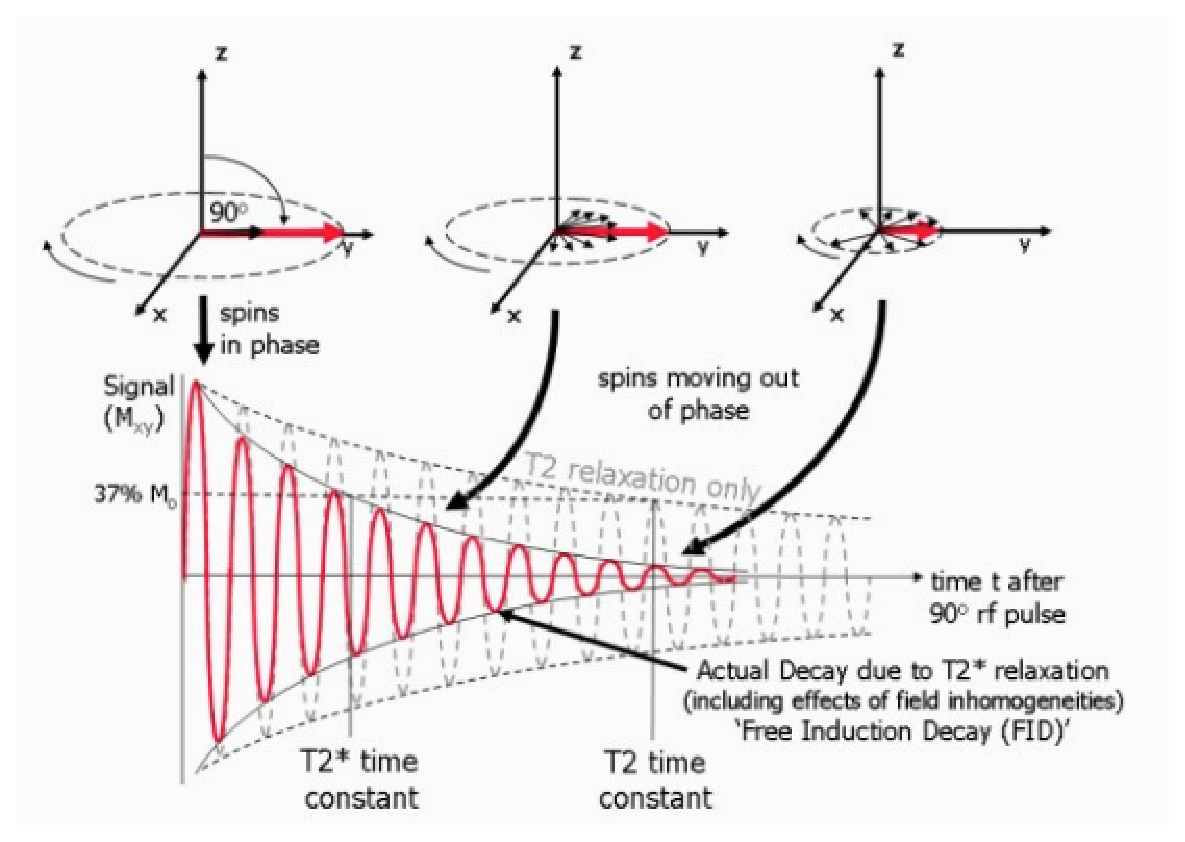
\includegraphics[width=0.7\textwidth]{contraste_T2}
   \caption{Relajación \Ttwo. Imagen provisional tomada de la tesis de Sasidhar Tandaki. \citep{tadanki2018}}
 \label{fig:T2}
 \end{figg}
\end{figure}


Existen dos tipos de desfasamientos producidos por inhomogeneidades de \Bzero: las reversibles y las irreversibles. El desfasamiento producido por las inhomogeneidades irreversibles se conoce com \Ttwostar (pronunciado \Ttwo estrella) \index{T2*|textbf}. Este desfasamiento reversible se suma al desfasamiento intrínseco del tejido, por lo que podemos considerar a \Ttwostar como la relajación \textit{observada} o efectiva, mientras que el \Ttwo es la relajación \textit{real}. La relación entre \Ttwo y \Ttwostar es

\begin{equation}
 1/T2^* = 1/T2 + 1/T2'
\end{equation}
donde $1/T2'= \Delta B_i$, es decir, las inhomogeneidades de \Bzero a lo largo de un voxel \footnote{http://mriquestions.com/t2-vs-t2.html}. Por lo tanto, \Ttwostar es \textit{siempre} más corto que \Ttwo.


Dada la variedad de composiciones tisulares, cada tejido tiene un \Ttwo (y \Ttwostar) particular, por lo que las curvas asociadas a cada uno de ellos son distintas (\figurapendiente). Tejidos altamente heterogéneos, o en cuyo interior existan elementos que provocan inhomogeneidades microscópicas de \Bzero, tendrán \Ttwo corto.

\section{Ecos}
\index{eco|textbf}
En la ecuación \ref{eq:T2} vimos que la señal obtenida es distinta dependiendo de en qué momento $t$ la evaluamos. Pero, ¿Cómo controlamos $t$? A través de la generación de un \textit{eco}, quizás uno de los trucos más asombrosos de la resonancia magnética, desarrollado por Erwin Hahn en la década de los 1950 y que debió haberle valido el premio Nobel \citep{mansfield2013long}. Igual que el eco de un grito emitido frente a una barranca, el eco de Hahn tiene como objetivo recuperar una señal que parecía perdida para siempre (en este caso, el FID). Siguiendo con las similitudes entre los ecos, es posible recibir un tren de ecos, cuyas magnitudes van decreciendo progresivamente ({\Large ¡Eco!} {\normalsize ¡Eco!} {\small ¡Eco!} {\tiny ¡Eco!}). Existen dos tipos de eco, que dependen de la manera en que se generan: eco de gradiente, y eco de spin.

\subsection{Eco de gradiente}
\index{eco de gradiente|textbf}
Dado que la frecuencia de precesión de un spin depende únicamente del campo magnético que experimenta, podemos hacer que un grupo de spins con localizaciones espaciales distintas precesen a diferentes frecuencias. Para ello, modulamos linealmente el campo magnético \Bzero, haciéndolo más potente de un lado, y menos potente del otro. Esto es también el pilar de la codificación espacial (Capítulo \ref{chapter_espacial}), pero por ahora lo usaremos para generar un eco de gradiente .\footnote{En resonancia hay varios trucos, y la mayoría se pueden usar en distintos escenarios para obtener distintos resultados, pero deben usarse en momentos específicos y no simultáneamente. Por ejemplo, un gradiente de campo magnético puede usarse primero para producir un eco de gradiente, y más adelante para realizar codificación espacial.} En presencia de un gradiente de campo magnético, los spins que se encuentran en un pixel presentarán una gama de frecuencias de precesión, lo que provocará que se desfasen fácilmente. Pero, como este desfasamiento fue controlado por el operador, es fácil de revertir mediante la inversión del gradiente. El lugar en el espacio donde antes había un campo magnético más potente es ahora más débil, y viceversa. La amplitud y dirección del gradiente del campo magnético debe ser invertida a la perfección para lograr un eco de gradiente (el segundo gradiente es un espejo del primero). Durante la presencia del primer gradiente, los spins se desfasan, y los que experimentan más campo magnético precesan más rápidamente y se adelantan a los lentos; al invertir el gradiente los spins que precesaban lento ahora lo hacen rápido y alcanzan a los ahora lentos (se refasan). Durante el primer gradiente, la suma vectorial que genera la señal va tendiendo a cero, pero durante el segundo gradiente su magnitud crece nuevamente, acercándose (pero no alcanzando) a su magnitud original. Así, la señal que se hubiera perdido como un FID se recupera como un eco. Puede incluso repetirse la inversión del gradiente, obteniendo ecos sucesivos, aunque éstos serán cada vez de menor magnitud. 

Los ecos de gradiente son capaces de recuperar un eco y son sensibles a los fenómenos relativos a \Ttwostar. Es decir, son capaces de recuperar la señal perdida por inhomogeneidades reversibles. Entre otras aplicaciones, los ecos de gradiente son de gran utilidad en la clínica para evaluar hemorragias, malformaciones arterio-venosas, y en la investigación son la piedra angular de la resonancia magnética funcional (Capítulo \ref{chapter_bold}), que es sensible al nivel de oxigenación de la hemoglobina (nótese como estos ejemplos comparten su dependencia con la sangre, y el \ce{^{26}Fe} en ella).

El operador puede decidir cuándo ejercer los gradientes de campo magnético, así como su duración. Esto determinará el momento en que se generará el eco, y por lo tanto, es utilizado para controlar la cantidad de contraste \Ttwostar presente en la imagen (ver sección \ref{sec:mod_contraste}).


\subsection{Eco de spin}
\index{eco de spin|textbf}
Los ecos de spin son capaces de recuperar mucho más señal que los ecos de gradiente, y son sensibles a procesos referentes a \Ttwo. Después del pulso de RF que desvía a \M, el eco se produce mediante un pulso de RF que voltea a \M 180\degrees. \figurapendiente


\section{Control del contraste}
El contraste es la diferencia de la intensidad de señal entre tejidos, y para fines prácticos la consideraremos como la diferencia de intensidad entre pixeles, en el supuesto de que distintos pixeles están ocupados por tejidos de composiciones distintas. Por ahora tendremos que ignorar cómo se realiza la codificación espacial (ver Capítulo \ref{chapter_espacial}), pero las descripciones que haremos se estarán llevando a cabo simultáneamente en todos los pixeles de la imagen. El concepto de contraste es fundamental, pues en las imágenes de resonancia magnética la intensidad de cada pixel está en unidades arbitrarias, y lo que importa es qué tan distintas son las intensidades entre pixeles.

En resonancia magnética existen múltiples mecanismos de contraste, lo que hace a la técnica muy versátil. Compárese con otros métodos de imagen, como la tomografía por rayos X, cuyo único mecanismo generador de contraste es la absorbancia de la radiación. Entre todos los mecanismos de contraste, los más importantes y siempre presentes son los relacionados a los fenómenos de relajación arriba descritos. El otro generador de contraste omnipresente es la cantidad de H en el tejido, que se conoce como \textit{densidad de protones} (el nivel de hidratación de un tejido). 

Al momento de adquirir imágenes de resonancia magnética, el operador puede decidir qué tanto influye uno u otro mecanismo generador de contraste. A las imágenes obtenidas se les suele llamar por el tipo de contraste que predomina. Por ejemplo, si el fenómeno de relajación longitudinal es el mayor generador de contraste, tendremos una imagen ``pesada'' o ``ponderada'' a \Tone (en inglés, \Tone-weighted). Para que un tipo de contraste predomine, habrá que minimizar la contribución de los otros. El único tipo de contraste que evidentemente no podremos controlar sin hacer daño al tejido (¡y participante!) es densidad de protones.

\subsection{Modulación de contraste \Ttwo}
\label{sec:mod_contraste}
Para maximizar la contribución de \Ttwo, debemos adquirir nuestra imagen justo cuando exista mayor diferencia entre las magnitudes de las señales de los diferentes tejidos (el $t$ de la ecuación \ref{eq:T2} que provea magnitudes disímiles). Si $t$ es muy corto, tendremos a todas nuestras señales con valores cercanos al máximo (a la izquierda en la Figura \ref{fig:contraste_T1_tejidos}). Si $t$ es demasiado largo, hemos perdido la señal de todos los tejidos por igual (hasta la derecha en la misma figura). Pero con $t$ medianamente largo, algunos tejidos brindarán mucha señal, mientras que otros brindarán poca, impartiendo contraste tipo \Ttwo. Contrariamente, para minimizar la contribución de \Ttwo debemos obtener nuestra señal en $t$ muy corto, de manera que todos los tejidos brinden el máximo de señal posible, con diferencias entre ellos dictaminadas únicamente por su densidad de protones. Como se detalla en la sección \ref{sec:imagenescomunes} y el Capítulo \ref{chapter_secuencias}, $t$ se controla mediante un parámetro conocido como \textit{tiempo de eco}, o TE. \index{TE (Tiempo de eco)}

\subsection{Modulación de contraste \Tone}
Entender la contribución de \Ttwo es relativamente sencillo, pues el fenómeno sucede en el plano $x,y$, que es de donde podemos captar señal. Pero \Tone sucede en el eje $z$, invisible para resonancia, lo que nos puede confundir. Para poder inyectar contraste tipo \Tone, no podemos hacer solo un experimento, debemos hacer varios. La rapidez con la que repitamos nuestros experimentos serán determinantes para que \Mz se vea modulada, y por tanto la señal que podemos poner en el plano $x,y$ mediante pulsos excitadores. En la ecuación \ref{eq:Tone} el parámetro $\tau$ indica qué tan rápido hacemos pulsos excitadores sucesivos, y comúnmente se le conoce como \textit{Tiempo de Repetición}, o TR (detallado en Capítulo \ref{chapter_secuencias}) \index{TR (Tiempo de repetición)|textbf}. Imaginemos, pues, que iniciamos nuestro experimento, y llamaremos a \Mz original como \Mzero. Tras un pulso que desvíe 90\degrees, \Mz partirá de cero e incrementará exponencialmente, y si lo dejamos mucho tiempo ($\tau\xrightarrow{}\infty$), crecerá tanto como \Mzero. Pero, si antes de que \Mz llegue a valer \Mzero aplicamos un nuevo pulso de RF, estaremos excitando únicamente la porción de \Mz que ya se había relajado, y la señal que obtendremos será entonces menor que la que hubiéramos obtenido con tan solo el primer pulso de RF. Hemos visto en el plano $x,y$ la consecuencia de no haber permitido la completa relajación longitudinal. El caso extremo de esta acción sería hacer un TR exageradamente corto. En este escenario, comenzaríamos con \Mz = \Mzero, tendríamos un primero pulso excitador (90\degrees, en este ejemplo), que llevaría a \Mz a un valor de cero; antes de recuperarse \Mz se recibiría un nuevo pulso excitador, y después otro, y así sucesivamente. El resultado sería que \Mz sería esencialmente obliterada y consecuentenemente no habría posibilidad de recibir señal (no se puede colocar a \M en el plano $x,y$ si no hay nada en \Mz). 

Hagamos una burda analogía para comprender cómo influye TR en el contraste \Tone. Recordemos el juego \textit{Whack-a-mole}, disponible en algunos restaurantes infantiles (Figura \ref{fig:whack}). En este juego, el objetivo es golpear con un mazo unos topos que salen de sus guaridas subterránas, asomando su cabeza. Algunos topos asoman su cabeza velozmente, mientras que otros son más lentos en su ascenso. Nos daremos una ventaja competitiva: en vez de usar un mazo y golpear individualmente a los topos, usaremos una tabla que los hundirá a todos simultáneamente. En este escenario imaginario, además, jugaremos a colectar a los topos (o fragmentos de ellos) en una canasta colocada a un costado del tablero. Para ello, un jugador utilizará un bat (o un temible machete) para guadañar a los topillos que se hayan aventurado a la superficie, lanzándolos hacia la canasta. La condición en este ejercicio (mental, afortunadamente), es que cada madriguera determina la velocidad de ascenso del topillo en cuestión, y el color de su camiseta (porque una vez que llegue a la canasta necesitamos saber de qué madriguera provino). Podemos determinar la frecuencia con la que damos un tablazo. Si lo hacemos exageradamente rápido, no permitiremos que ningún topillo asome su cabeza, y no recibiremos nada en la canasta (nuestro sádico amigo estará haciendo \textit{strikes} a cada intento entre tablazos). Si, por el contrario, tardamos mucho tiempo entre tablazos, todos los topillos con camisetas de distinto color estarán equitativamente representados en la canasta del horror. Pero existirá un punto intermedio en el ritmo de los tablazos, de manera que los topillos con ascenso rápido llegarán completos a la canasta, recolectaremos fragmentos de aquéllos con ascenso intermedio, y los demasiado veloces no estarán muy representados. En esta analogía, el ritmo de los tablazos es el TR, la velocidad de ascenso de los topillos es el \Tone del tejido, y el color de los topillos es la codificación espacial (Capítulo \ref{chapter_espacial}. Podemos ver nuevamente que la excitación repetida modula la magnitud de \Mz y por ende la señal potencial recibida.


\begin{figure}[htb]
\begin{figg}
   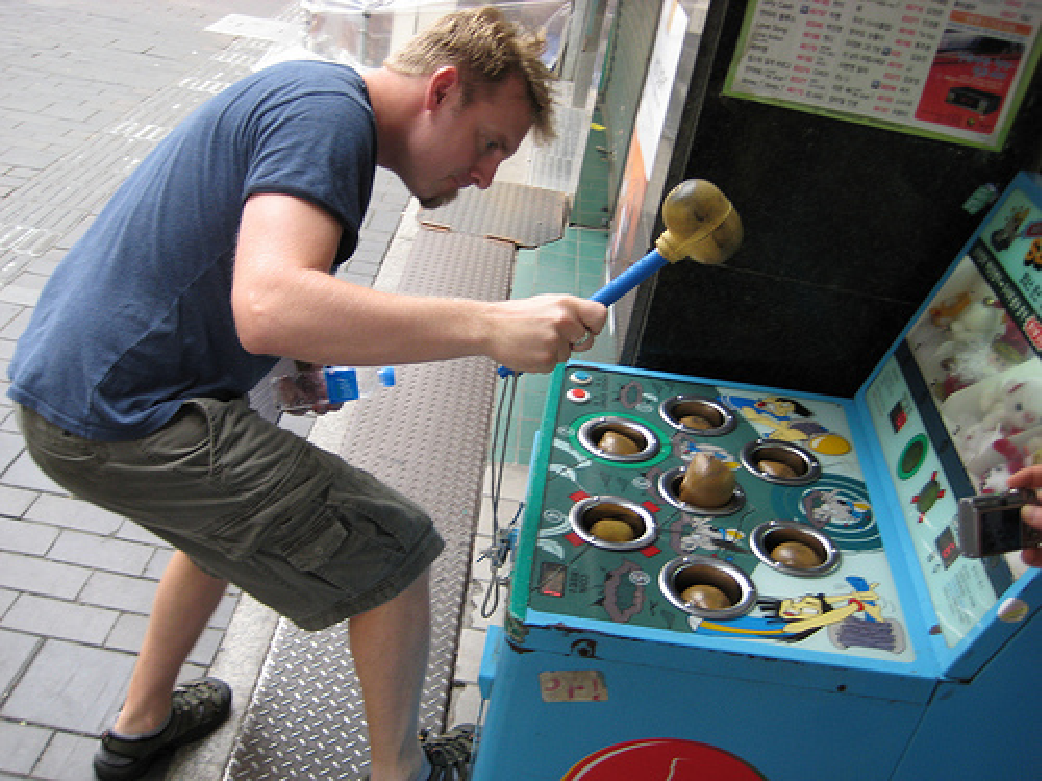
\includegraphics[width=0.7\textwidth]{whack}
   \caption{Juego de \textit{Whack-a-mole}.}
 \label{fig:whack}
 \end{figg}
\end{figure}


\subsection{Los tres tipos de imágenes más comunes}
\label{sec:imagenescomunes}
Sabiendo modular la contribución del contraste \Tone y \Ttwo, y admitiendo que nada podemos hacer por la densidad de protones en un tejido, tenemos oportunidad de generar cuatro diferentes imágenes (Figura \ref{fig:diferentes_contrastes}). De ellas, solo tres de ellas son de utilidad clínica, pues es difícil interpretar una imagen pesada simultáneamente a los tres mecanismos de contraste.


\subsubsection{Imagen pesada a \Tone}
Para hacer una imagen con este contraste, debemos maximizar la contribución de la relajación longitudinal, a la vez que minimizamos la contribución de la relajación transversal. Debemos, entonces, utilizar un TR tal que no sature la señal (no demasiado corto, recordemos a los topillos), ni tan largo que permita la relajación total de todos los tejidos. Le llamaremos un TR corto, entendiendo largo en el contexto del \Tone propio del tejido. Por ejemplo, para tejidos con valores \Tone en el rango de [400 1500] s, un TR largo sería alrededor de esos mismos valores, o incluso menor.

Para minimizar la contribución de \Ttwo, usaremos un TE corto. De esta forma, estaremos adquiriendo nuestra señal antes de que se exprese un desfasamiento diferencial entre tejidos (los valores de los diferentes tejidos son muy similares entre ellos en la parte más izquierda de la \figurapendiente. Uno puede pensar que también son muy similares entre ellos en la parte más a la derecha de la misma figura, y tendría razón en cuanto a las mínimas diferencias entre ellos, pero tendríamos muy poca o nula señal, con lo que nuestra imagen sería inútil.

Maximizando entonces la contribución de \Tone mediante un TR corto, y minimizando la contribución de \Ttwo con un TE corto, obtendremos una imagen pesada a \Tone. La substancia blanca, teniendo el \Tone más corto, logra brindar mucha señal y es brillante, mientras que el líquido-cefalo-raquídeo presenta el patrón inverso, con la substancia gris con intensidad intermedia.

\subsubsection{Imagen pesada a \Ttwo}
Ahora debemos hacer el ejercicio inverso al anterior. Minimizaremos la contribución de \Tone dejando que todos los tejidos se relajen totalmente, lo que podremos lograr dándoles suficiente tiempo para que el fenómeno de relajación suceda, con un TR largo. Nuevamente, entendemos largo en el contexto del \Tone de los tejidos de interés, y un TR largo es habitualmente unas dos o tres veces más largo que el \Tone más largo (formalmente deberíamos esperar una eternidad TR $\xrightarrow{}\infty$, pero nadie tiene tiempo para ello).

Para maximizar la influencia de la relajación transversal, dejaremos que ésta suceda con un TE largo. Un TE muy corto, como vimos, no permite la diferenciación de las intensidades de señal entre tejidos. Un TE largo ronda o excede un poco los valores de \Ttwo de los tejidos, pero no va más allá de tres veces dicho valor, porque para entonces todos los tejidos ya tendrán totalmente desfasados sus spins, y no podrán darnos nada de señal. Los tejidos que se relajan lentamente, como el líquido cerebro-raquídeo, brindarán mucha señal, mientras que los que se relajan rápido, como la substancia gris, serán más obscuros.

\subsubsection{Imagen pesada a densidad de protones}
Siendo la densidad de protones el único mecanismo de contraste que no podemos modular con ningún parámetro, la estrategia será minimizar la influencia de los otros dos mecanismos de contraste, \Tone y \Ttwo. Repasando la información que acabamos de revisar, sabemos que podemos minimizar la contribución de \Tone con un TR largo (todos los tejidos se relajarán totalmente), mientras que un TE corto minimizará la contribución de \Ttwo (los spins de todos los tejidos están aún todos en fase). Por lo tanto, la diferencia en la intensidad entre los diferentes tejidos estará dictada primordialmente por sus diferentes niveles de hidratación. El agua del líquido cerebro-raquídeo será muy brillante, mientras que el hueso del cráneo será el tejido más obscuro en una imagen de cerebro.



\begin{figure}[htb]
\begin{figg}
   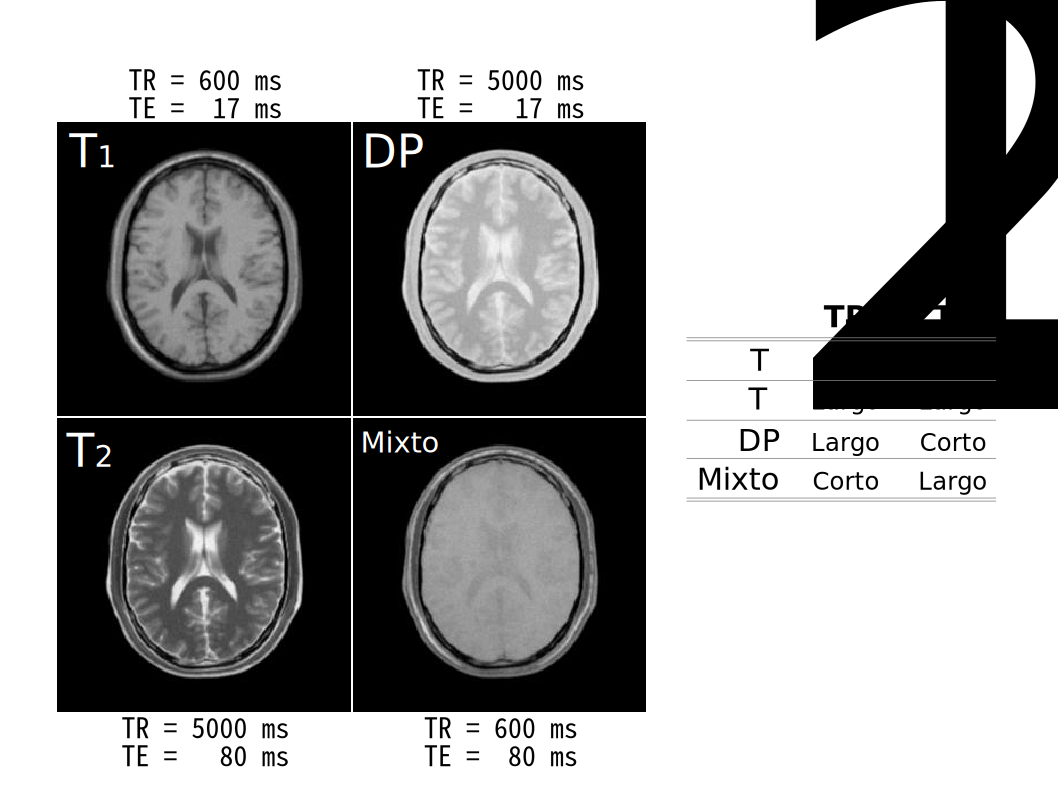
\includegraphics[width=0.7\textwidth]{diferentes_contrastes}
   \caption{Imágenes pesadas a diferentes contrastes obtenidas en un resonador de 3 teslas. Para cada imagen se indica el mecanismo de contraste que predomina; por ejemplo la imagen pesada a \Tone está indicada como \Tone. Adyacente a cada imagen se indican los parámetros TR y TE correspondientes. La tabla de la derecha resume en términos cualitativos los valores TR y TE para obtener cada tipo de imagen. La imagen con contraste mixto es difícil de interpretar y de poca utilidad. TR: tiempo de repetición; TE: tiempo de eco; DP: densidad de protones.}
 \label{fig:diferentes_contrastes}
 \end{figg}
\end{figure}



% Como se mencionó en el capítulo anterior, cuando se aplica un campo magnético externo o Radiofrecuencia (\Bone) superior al campo magnético principal (\Bzero),  nuestros spins o protones de hidrógeno comienzan a precesar en dirección a este nuevo campo magnético.
% 
% ¿ Pero que ocurre cuando este campo magnético externo  se “apaga”?
% 
% Es lógico pensar que los spins regresarán a B0 (su posición original sobre el eje \textit{z}),  pero es la trayectoria que realizan la que es de interés para la obtención de una Imagen de Resonancia Magnética. A este fenómeno se le conoce como Relajación y es el proceso que llevan a cabo los spins para regresar a su sitio de origen en este caso R0 también conocido como \Mz, mismo que logran liberando energía en su trayectoria. 
% 
% La relajación ocurre debido a que los spins desprenden la energía que habían absorbido al entrar en resonancia.
% 
% 
% En la Relajación de estos spins ocurren dos fenómenos simultáneamente, el primero llamado relajación longitudinal o \Tone y el segundo conocido como relajación transversal o \Ttwo. 
% 
% \section{RELAJACIÓN LONGITUDINAL (\Tone)}
% 
% Llamada de esta forma porque es el fenómeno que ocurre sobre el eje \textit{z}, es una constante en el tiempo de la trayectoria del spin, para retomar su lugar sobre \Mzero.
% Se define como: ``El tiempo que tarda en recuperarse el 63\% del \Mz original''
% 
% 
% Tras  el pulso de radiofrecuencia nuestro spin cambió su eje magnético al plano de las \textit{x}. Esta es la razón que provoca  que parezca pequeño sobre el eje \textit{z}.
% 
% Una vez que el pulso de radiofrecuencia se elimina, el spin retomará su dirección. Comienza entonces a precesar más lentamente y a regresar a \Mz por lo que este comienza a crecer conforme los segundos transcurren (\Tone). Finalmente el protón de Hidrógeno regresa a su posición original provocado por el campo magnético principal (\Mz).
% 
% 
% El fenómeno de relajación T1 se define como:
% ``El tiempo que tarda el spin en recuperar su campo magnético original (\Mz) en un 63\%''
% 
% En la representación gráfica se observa como una exponencial ascendente.
% 
% 
% 
% \section{RELAJACIÓN TRANSVERSAL (\Ttwo)}
% 
% Al igual que el concepto antes descrito, el nombre es mera cuestión de lógica, se le denomina Relajación Trasversal por que ocurre sobre el plano \textit{x,y}. Otra forma en la que se conoce al \Ttwo es como Relajación Spin- Spin o \Ttwop ya que el fenómeno se observa en un conjunto de protones de hidrógeno. En el caso de la relajación \Ttwop  la representación gráfica nos habla de una caída en la señal original por lo que se define de la siguiente forma:
% ``Tiempo en el cual solamente queda el 37\%de la señal \Mxy original, es decir de la emitida por el pulso de radiofrecuencia''
% 
% 
% 
% Comencemos por entender que el T2 es el resultado de la actividad de varios spins. En un inicio como se ha venido mencionando la Radiofrecuencia (\Mzero) que provocó que nuestros spins cambiaran del eje \textit{z} al plano \textit{x,y}, también provocó que varios spins precesaran al mismo tiempo, es decir todos giraban a la misma frecuencia. 
% 
% 
% Al suspender \Mzero, cada spin comienza a relajarse a su propio tiempo , y poco a poco cada uno regresa a su \Mzero, esto provoca que se desfasen uno del otro.
% 
% 
% \subsection{Fenómeno \Ttwostar}
% 
% El desfase es provocado por inhomogeneidades en el campo magnético que experimentan los protones de hidrógeno y debido a que ocurren en el fenómeno \Ttwo se les conoce como \Ttwostar, estas inconsistencias pueden ser de dos tipos dependiendo de que las genere:
% 
% \begin{description}
%  \item [Intrínsecas]  Suceden por acumulación de metales en el paciente.
%  \item [Extrínsecas]  Se deben a inhomogeneidades en el campo magnético del resonador,  presencia de objetos metálicos, e incluso productos para el cabello.
% \end{description}
% 
% 
% 
% 
% \section{Contraste}
% 
% 
% El contraste se define como: ``la diferencia entre la intensidad de señal entre dos muestras, secundario a las propiedades magnéticas de las mismas''.
% 
% Tras el pulso de radiofrecuencia inicial, la energía que se libera de nuestro Spin en los fenómenos de \Tone y \Ttwo (\Ttwop - \Ttwostar),  es captada por una antena que codifica la señal en nuestro aparato de resonancia magnética, y que se puede observar como una ``disminución en la señal'' es decir un decremento de nuestro pulso inicial hasta el regreso a su estado basal, a esta caída se le conoce como Free Induction Decay (FID).
% 
% 
% 
% La antena que capta la señal de radiofrecuencia, lo hace simultáneamente para todos los spins que se le diga que debe captar señal, por lo que al revisar esta señal ``cruda'' tendremos entremezclado la señal de todos nuestros spins, posteriormente estas señales podrán ser diferenciadas mediante un análisis de Fourier. 
% 
% 
% 
% Algo que debemos tomar en cuenta es que este proceso está sucediendo en los tejidos y que la conformación de estos es muy diferente; ya sea que hablamos de sangre, grasa, hueso etc. Debido a lo diverso de la composición de las estructuras que rodean a nuestro protón, la liberación de esta energía y el retorno a su campo magnético original (\Mz) será distinta para cada protón al igual que la señal que captaremos con nuestra antena.
% 
% El análisis de estas señales es lo que nos permitirá diferenciar estructuras dependiendo si al ``leer'' estas señales lo hacemos más influenciados por el fenómeno \Tone o \Ttwo, a esto se le denomina de forma genérica \textit{potenciar} se dice que nuestra imagen esta potenciada a uno de estos fenómenos de resonancia magnética según lo observado en nuestra imagen final , es justo este proceso el que nos permite crear el contraste de las estructuras aprovechando su comportamiento bajo resonancia magnética.
% 
% 
% \subsection{Imágenes potenciadas a densidad de protones}
% 
% Como se ha venido mencionando, la magnetización de nuestros spins está influenciada por la densidad de los mismos en la muestra que se esté estudiando. De ahí que podamos jugar con la manera en la que observamos estas imágenes, y para el caso de las imágenes potenciadas en densidad se sigue la siguiente regla:
% 
% ``La intensidad de la imagen es directamente proporcional a la densidad de protones de hidrógeno''
% 
% ¿Qué quiere decir esto? que al hacer la lectura de nuestra imagen el lugar donde se reciba más señal será donde existan más protones de hidrógeno. Se sabe que los tejidos tienen distintas densidades, dependiendo si son grasa, hueso, LCR, etc.
% 
% 
% Estas imágenes se obtienen al enviar un pulso de radiofrecuencia (RF) de 90º  y esperando un tiempo largo (tiempo de repetición o TR) antes de dar nuestro siguiente pulso, para permitir que los tejidos envíen la señal de sus spins.
% 
% 
% \subsection{Imágenes potenciadas a \Tone}
% 
% Cuando hablamos de imágenes potenciadas a \Tone nos referimos a que al momento de codificar nuestra imagen lo hicimos tomando en cuenta las propiedades de la relajación longitudinal (\Tone) de nuestros spins y que se ha trabajado bajo la siguiente premisa:
% 
% ``Mientras más rápido libere energía nuestro spin, más rápido regresará a \Mz  y mayor será la intensidad de nuestra señal''
% 
% Un ejemplo de ello es la grasa la cual  se relaja fácilmente ya que su densidad de hidrógenos no es tan alta por lo que su señal es captada más rápido lo que se traduce en mayor señal o contraste blanco.
% 
% 
% Para obtener imágenes potenciadas a \Tone se da un solo pulso de radiofrecuencia de 90\degrees y se realiza la lectura una vez que los spins hayan vuelto a su eje magnético principal.
% 
% 
% \subsection{Imágenes potenciadas a \Ttwo y \Ttwostar}
% 
% Para el caso de las imágenes potenciadas a \Ttwo y \Ttwostar la señal la conseguimos cuando nuestros spins se encuentran sobre el plano \textit{x,y}, captando la señal por medio de nuestra antena. 
% 
% Para que la señal sea más duradera nosotros damos el primer pulso de radiofrecuencia para llevar a todos nuestros spins a \Mx  y antes de que regresen a su campo magnético original , se les aplica otro pulso de 180\degrees  el cual provoca que nuevamente se encuentren y vuelvan a refasarse.
% 
% 
% 
% 
